\documentclass[a4paper,12pt]{article}
\usepackage{/home/rweye/Documents/Overleaf/Styles/Cours}

\title{\vspace{-1cm}\large 
	\begin{tabular}{|m{7cm}|>{\centering}m{6cm}|>{\centering\arraybackslash}m{4cm}|}
		\hline
		 Nom :& \textbf{\textsc{2GT DS Lentilles}} &  Note\\
		 &&\\
		 Prénom : &&\\
		\hline
\end{tabular}}
\date{}


\begin{document}
	\maketitle
	\vspace{-3cm}
\section*{Exercice 1 : Lentilles minces convergentes}
Pour chacune des lentilles suivantes, dire s'il s'agit ou non d'une lentille mince convergente et justifier votre réponse.\\

\begin{tabular}{|>{\centering}m{2.5cm}|>{\centering}m{2.5cm}|>{\centering}m{2.5cm}|>{\centering}m{2.5cm}|>{\centering}m{2.5cm}|>{\centering\arraybackslash}m{2.5cm}|}
	\hline
	1&2&3&4&5&6\\
	\hline
	
\includegraphics[trim={ 0 0 21cm 0},clip,scale=.25]{2GT_DS_lentille_Fig1.png}&
\includegraphics[trim={ 5cm 0 17cm 0},clip,scale=.25]{2GT_DS_lentille_Fig1.png} & 
\includegraphics[trim={ 9cm 0 12cm 0},clip,scale=.25]{2GT_DS_lentille_Fig1.png} & 
\includegraphics[trim={ 13cm 0 8cm 0},clip,scale=.25]{2GT_DS_lentille_Fig1.png}& 
\includegraphics[trim={ 18cm 0 5cm 0},clip,scale=.25]{2GT_DS_lentille_Fig1.png}& 
\includegraphics[trim={ 21cm 0 0cm 0},clip,scale=.25]{2GT_DS_lentille_Fig1.png}\\
	\hline
	&&&&&\rule[4cm]{0cm}{0cm}\\
	\hline
\end{tabular}


\section*{Exercice 2 : Image d'un objet par une lentille}
Un objet $AB$ de taille \SI{1,5}{cm} est placé \SI{5,0}{cm} avant le centre optique $O$ d'une lentille convergente, de distance focale $f' = \SI{2,0}{cm}$ (AB est perpendiculaire à l'axe optique)?
\begin{enumerate}
	\item Définir la distance focale d'une lentille mince convergente.
	\item Construire l'image $A'B'$ de l'objet $AB$ en utilisant les trois rayons particuliers. On prendra pour échelle \SI{1}{cm} sur la copie = \SI{0,5}{cm} réels.(Sur partie millimétrée au dos)
	\item Calculer le grandissement $\gamma$ et indiquer le sens de l'image.
	\item Proposer une autre méthode pour calculer $\gamma$ et comparer les résultats à la réponse précédente.
\end{enumerate}

\section*{Exercice 3: L'\oe il et la vision}
\begin{enumerate}
	\item L'\oe il peut être modélisé par 3 éléments d'optique, représenter ces trois éléments sur un schéma modélisant un \oe il.
	\item Associer à chacun de ces éléments une partie de l'anatomie de l'\oe il.
	\item Un \oe il sans défaut ajuste sa distance focale de manière à voir nettement des objets proches de lui. Sa limite est d'environ \SI{25}{cm} (en dessous il n'est pas possible avec un seul \oe il d'avoir une image nette d'un objet). Représenter sur un schéma la situation où un objet ($AB = \SI{10}{cm}$ est situé à \SI{20}{cm} de l'\oe il et expliquer en construisant l'image pourquoi il n'est pas possible de voir nettement cet objet. (Échelle : \SI{5}{cm} réels = \SI{1}{cm} sur le schéma, sur partie millimétrée au dos)
\end{enumerate}

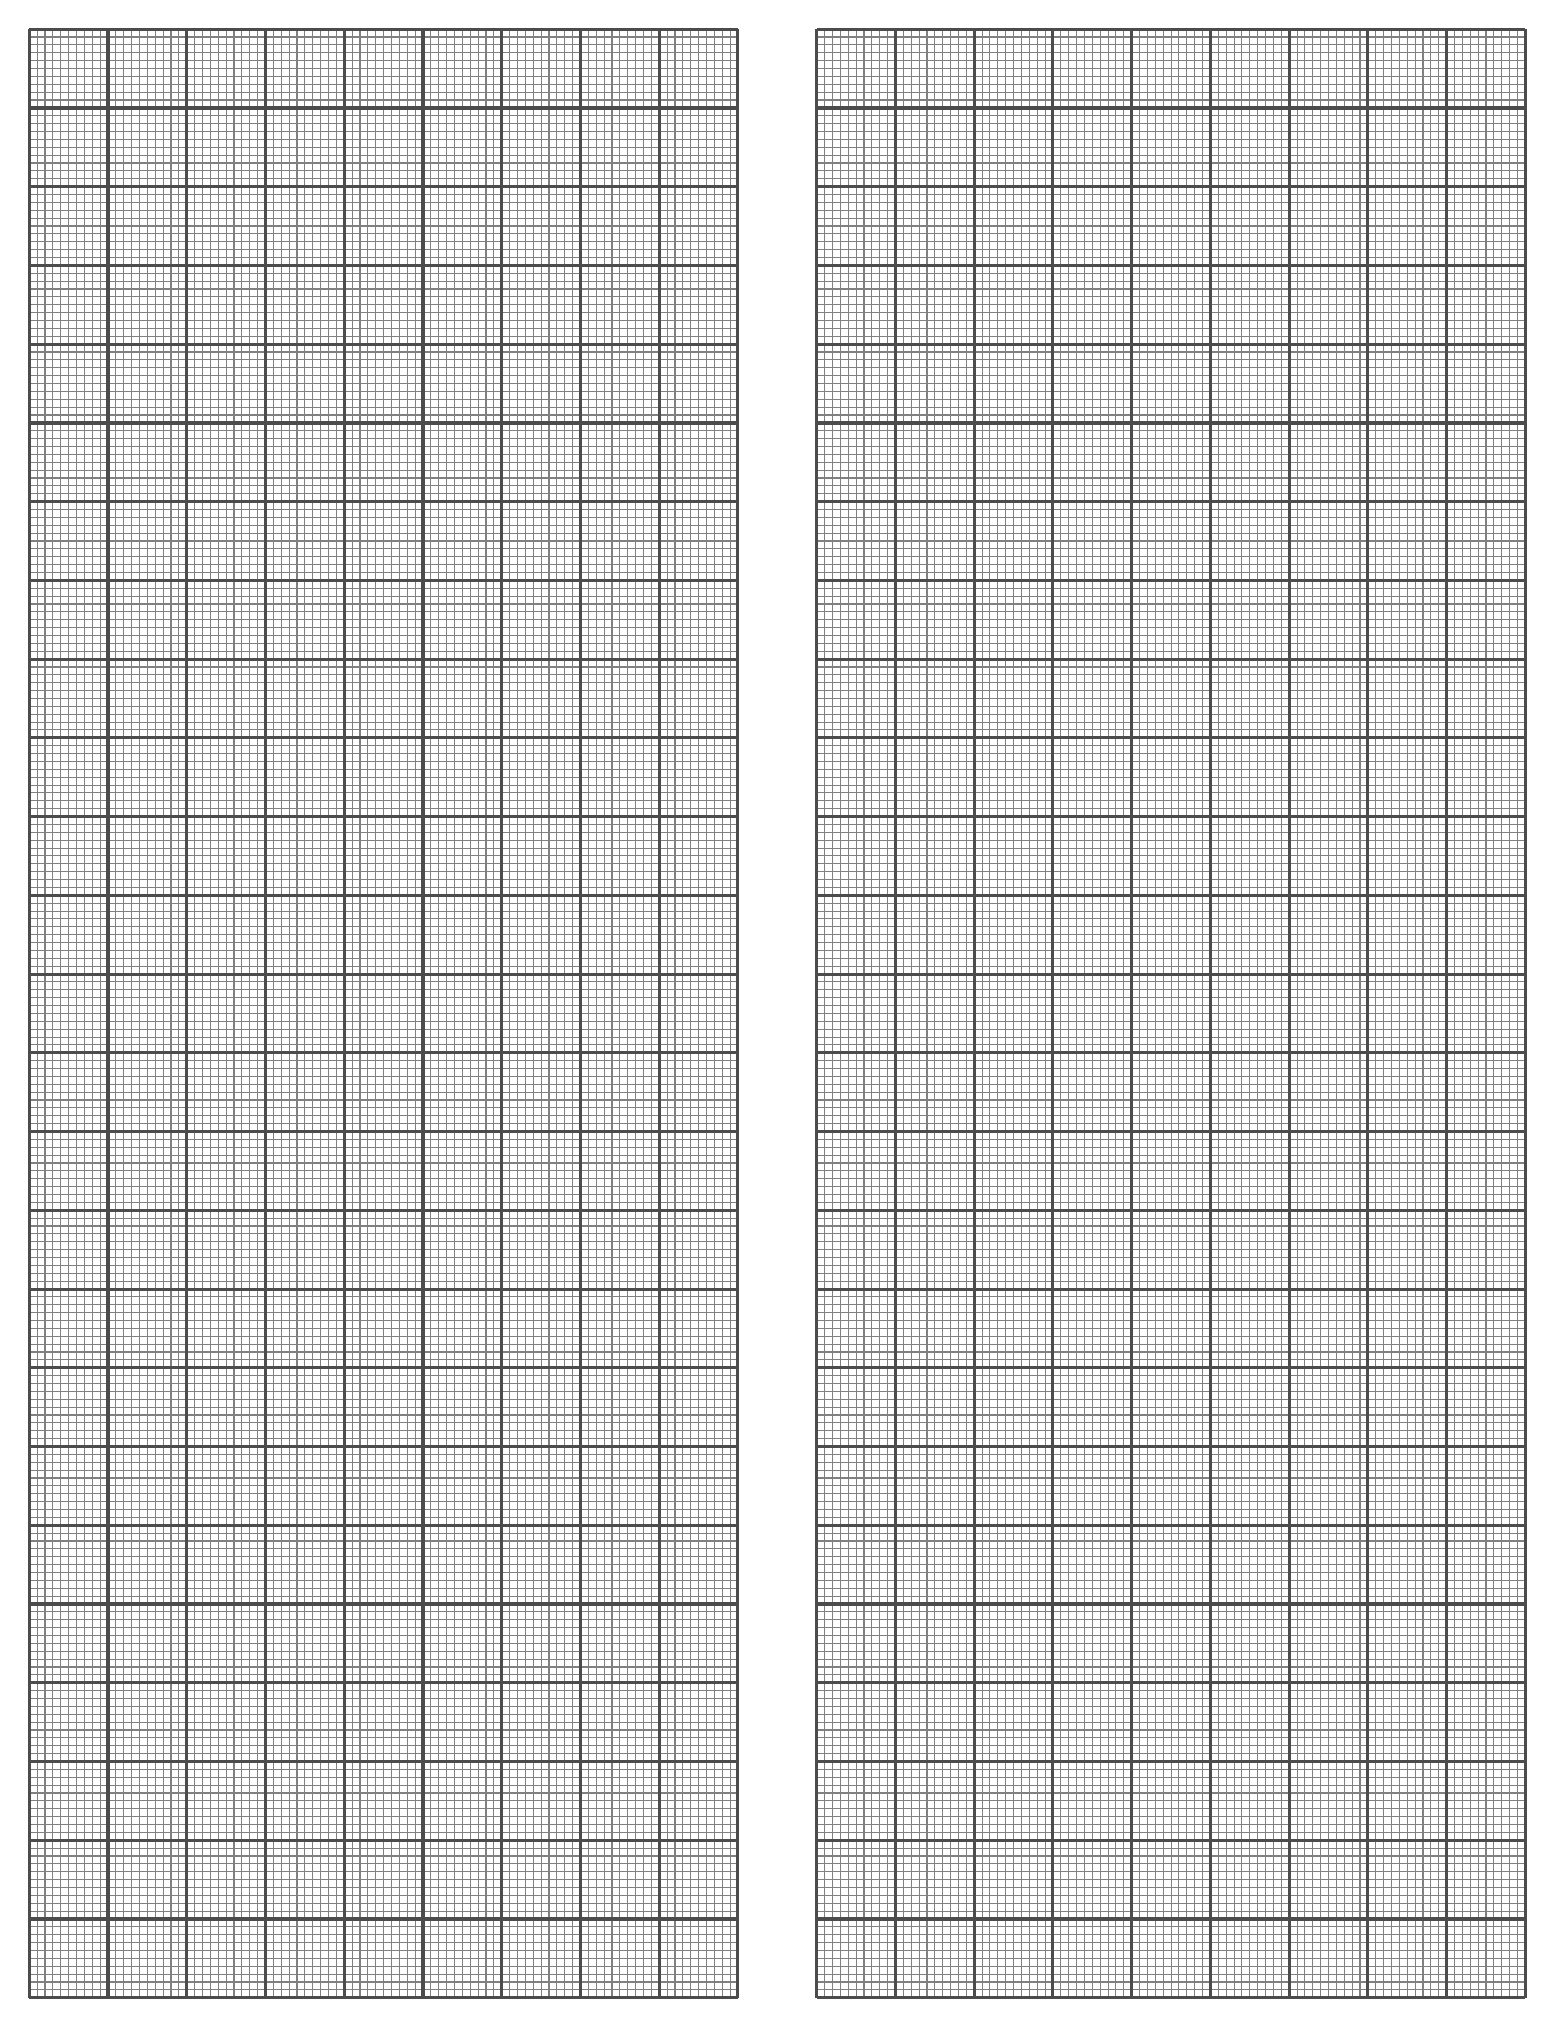
\begin{tikzpicture}
	\draw[gray] (0,0) grid[step=.1cm](9,25);
	\draw[black!70][line width= .04cm] (0,0) grid(9,25);
	
	\draw[gray] (10,0) grid[step=.1cm](19,25);
	\draw[black!70][line width= .04cm] (10,0) grid(19,25);
	
\end{tikzpicture}
\end{document}